%%%%%%%%%
\section{Event selection and categorization}\label{sec:finalselection}
%%%%%%%%%

Events are selected online with triggers requiring either one muon or electron (Sections~\ref{subsec:eletrigger} and~\ref{subsec:mutrigger}).
Several requirements are then applied offline to the selected events to enhance the analysis sensitivity as described in the following.\\
%The strategy is slightly different for the two analyses described in this work and they will both summarized in the following.

The two analyses described in this work feature the same selection strategy on the leptonic part of the final state.
Both analyses require exactly one muon or one electron satisfying certain \pt and $\eta$ requirements and passing 
the high-\pt lepton identification criteria described in Sections~\ref{subsec:muonid} and~\ref{subsec:eleid}.
As summarized in Tables~\ref{tab:cutsummaryWH} and~\ref{tab:cutsummaryWV}, the only difference is in the \pt threshold of the lepton which is higher for the 13\TeV data analysis
to match the increase in the trigger threshold. The offline reconstructed \pt of the electron must be greater than 90 (120)\GeV for the 8 (13)\TeV data analysis, where the trigger reaches the plateau.
This is required in order to avoid any bias on the distributions due to the turn-on of the trigger efficiency curve and its description in simulation.
%In fact, this choice is made to simplify the analysis avoiding the need for modelling possible biases in the distributions due to the turn-on of the trigger efficiency curve.
%In fact, this choice is made to simplify the analysis avoiding the need for modelling the turn-on of the trigger efficiency curve and, as a consequence, reducing the associated systematic uncertainties.
Reconstructed electrons must have $|\eta| < 2.5$ and also be located outside of the overlap region between the ECAL barrel and endcaps, because the reconstruction of an electron object in
this region is not optimal. In a similar way, the offline reconstructed \pt of the muon must be greater than 50 (53)\GeV for the 8 (13)\TeV analysis, and within $|\eta| < 2.1$ as a consequence of the trigger criteria.
Events with additional well-identified muons and/or electrons are rejected to avoid contamination from events containing $\PZ\to\ell\ell$ decays.\\

\begin{table}[!htb]
\begin{center}
\caption{Summary of the final selection for the 8\TeV data analysis in the $\ell\nu\bbbar$ decay channel.}
\label{tab:cutsummaryWH}
\begin{tabular}{lc}
\hline
\multicolumn{1}{c}{\textbf{Selection}} & \textbf{Value}\\
\hline
\multicolumn{1}{c}{Lepton selection}\\
\cline{1-1}
Electron & $\pt > 90\GeV$\\
              & $|\eta| < 2.5$ except [1.44, 1.57] range\\
Muon    & $\pt > 50\GeV$\\
             & $|\eta|<2.1$\\
\hline
\multicolumn{1}{c}{AK5 jet selections}\\
\cline{1-1}
Jet \pt &  $\pt >30\GeV$\\
Jet $\eta$  & $|\eta|<2.4$\\
\hline
\multicolumn{1}{c}{\ETmiss selections}\\
\cline{1-1}
\ETmiss (electron channel) &  \ETmiss$>80~\GeV$\\
\ETmiss (muon channel) & \ETmiss$>40~\GeV$\\
\hline
\multicolumn{1}{c}{Boson selections}\\
\cline{1-1}
$\PW\to\ell\Pgn$ & $\pt > 200\GeV$\\
$\PH\to\bbbar$ (CA8 jet) & $\pt > 200\GeV$\\
 & $|\eta| < 2.4$ except [1.0, 1.8] range\\
Back-to-back topology & $\Delta R (\ell , \PH_{\bbbar}) > \pi/2$ $\,$\\
                      & $\Delta \phi (\PH_{\bbbar} , \ptvecmiss)>2$\\ 
                      & $\Delta \phi (\PH_{\bbbar} , \PW_{\ell\Pgn})>2$\\
Diboson invariant mass & $\mWH > 0.7\TeV$\\                      
\hline
\multicolumn{1}{c}{H tagging selections}\\
\cline{1-1}
pruned-jet mass       & $110 < \mJ < 135\GeV$\\
Combined b-tagging cut	& 2 CSVL b-tagged subjets if $\Delta R(\mathrm{subjets}) > 0.3$\\
			& 1 CSVL b-tagged CA8 jet if $\Delta R(\mathrm{subjets})$\\ 
\hline
\multicolumn{1}{c}{\ttbar rejection}\\
\cline{1-1}
B-tag veto      & no CSVM b-tagged AK5 jet\\
		& within $\Delta R (\PH_{\bbbar}, AK5) = 0.8$\\
Top quark mass veto	& $m_\mathrm{top}^\mathrm{l} < 120~||~m_\mathrm{top}^\mathrm{l} > 240$\\
		& $m_\mathrm{top}^\mathrm{h} < 160~||~m_\mathrm{top}^\mathrm{h} > 280$\\
\hline
\end{tabular}
\end{center}
\end{table}

\begin{table}[!htb]
\begin{center}
\caption{Summary of the final selection for the 13\TeV data analysis in the $\ell\nu\qqbar$ decay channel.}
\label{tab:cutsummaryWV}
\begin{tabular}{lc}
\hline
\multicolumn{1}{c}{\textbf{Selection}} & \textbf{Value}\\
\hline
\multicolumn{1}{c}{Lepton selection}\\
\cline{1-1}
Electron & $\pt > 120\GeV$\\
              & $|\eta| < 2.5$ except [1.44, 1.57] range\\
Muon    & $\pt > 53\GeV$\\
             & $|\eta|<2.1$\\
\hline
\multicolumn{1}{c}{AK4 jet selections}\\
\cline{1-1}
Jet \pt &  $\pt >30\GeV$\\
Jet $\eta$  & $|\eta|<2.4$\\
\hline
\multicolumn{1}{c}{\ETmiss selections}\\
\cline{1-1}
\ETmiss (electron channel) &  \ETmiss$>80~\GeV$\\
\ETmiss (muon channel) & \ETmiss$>40~\GeV$\\
\hline
\multicolumn{1}{c}{Boson selections}\\
\cline{1-1}
$\PW\to\ell\Pgn$ & $\pt > 200\GeV$\\
$\PV\to\qqbar$ (AK8 jet) & $\pt > 200\GeV$\\
 & $|\eta| < 2.4$\\
Back-to-back topology & $\Delta R (\ell , \PV_{\qqbar}) > \pi/2$ $\,$\\
                      & $\Delta \phi (\PV_{\qqbar} , \ptvecmiss)>2$\\ 
                      & $\Delta \phi (\PV_{\qqbar} , \PW_{\ell\Pgn})>2$\\
Diboson invariant mass & $\mWV > 0.7\TeV$\\                       
\hline
\multicolumn{1}{c}{V-tagging selections}\\
\cline{1-1}
pruned-jet mass       & $ 65 < \mJ < 105\GeV$\\
2- to 1-subjettiness ratio & $\nsubj <$ 0.6\\
\hline
\multicolumn{1}{c}{\mJ categories}\\
\cline{1-1}
WW-enriched   & $ 65 < \mJ < 85\GeV$ \\
WZ-enriched   & $ 85 < \mJ < 105\GeV$\\
\hline
\multicolumn{1}{c}{\ttbar rejection}\\
\cline{1-1}
B-tag veto      & no CSVM b-tagged AK5 jet\\
		& within $\Delta R (\PV_{\qqbar}, AK5) = 0.8$\\				       
\end{tabular}
\end{center}
\end{table}

The requirements \ETmiss $>$ 40 and $>$ 80\GeV are applied, respectively, in the muon and electron channels.
The threshold is higher in the electron channel to further suppress the larger background from multijet processes expected at low values of \ETmiss due to jets misidentified as electrons.
This background is expected to be negligible in the muon channel, for which a lower \ETmiss threshold can be used to preserve a higher efficiency for a low-mass signal.
The identified lepton and the \ETmiss are used to reconstruct the W $\rightarrow\ell\Pgn$ candidate as described in Section~\ref{sec:leptonicW},
which is required to have $\pt > 200\GeV$.\\

A different strategy is instead used in the two analyses, for the hadronic part of the final state.
As described in Section~\ref{sec:jets}, the CA8 and AK8 algorithms are used to reconstruct the H- and V-jet candidates in the 8 and 13\TeV analysis, respectively.
In both cases the jet is required to have $\pt > 200\GeV$ and $|\eta| < 2.4$. %In addition, jets within $\Delta R < 0.8$ of any well-identified electron or muon are not used in the analysis.
For CA8 jets, the pseudorapidity region $1.0 < |\eta| < 1.8$ is excluded corresponding to the barrel-endcap transition region of the silicon tracker where the reconstruction of tracks is not optimal (Section~\ref{subsec:jetsreco}).
The probability of signal events with jets outside this region is 80\% (92\%) for a resonance mass of 1.0 (2.5)\TeV.

The 8\TeV analysis aims at isolating events with a high-\pt Higgs boson decaying to \bbbar and the H tagging algorithm described in Section~\ref{sec:htagging} is applied.
The H tagging requires the selected CA8 jet to have pruned mass in the range $110 < \mJ < 135\GeV$. Furthermore, the subjets are required to be b-tagged with the CSVL algorithm if their angular distance $\Delta R < 0.3$.
Otherwise, b tagging is applied to the whole CA8 jet using the same algorithm.

The 13\TeV analysis is instead focused on events with a high-\pt V boson decaying to \qqbar and the V-tagging algorithm described in Section~\ref{sec:htagging} is applied in this case.
The pruned-jet-mass window is shifted down to the V-boson mass, requiring the selected AK8 jet to have pruned mass in the range $65 < \mJ < 105\GeV$.
Furthermore, the V jet is required to have $\nsubj < 0.6$.
Finally, the V jet is deemed a W-boson candidate if its pruned mass falls in the range 65--85\GeV, while it is deemed a Z-boson candidate if it falls in the range 85--105\GeV instead.
This categorization has been added on the top of the V-tagging requirements on the \mJ to enhance discrimination between resonances with different charge and spin. 
Indeed, the first category, referred to as  ``WW-enriched'', has a higher sensitivity for resonances such as the neutral spin-2 graviton or the neutral spin-1 \Zpr decaying to WW, where a W jet is expected.
The second category, referred to as ``WZ-enriched'', is instead optimized for resonances such as the charged spin-1 \Wpr decaying to WZ, where a Z jet is expected.\\

In addition, there are specific topological selection criteria chosen for both the analyses. 
It is required that the two V bosons from the decay of a massive resonance are approximately back-to-back:
the $\Delta R$ between the lepton and the signal jet is greater than $\pi/2$; the $\Delta\phi$ between the vector \ptvecmiss and the signal jet,
as well as between the $\PW\to\ell\Pgn$ and signal jet candidates, are both greater than 2 radians.

To reduce the level of the \ttbar background, events with one or more reconstructed AK5 (or AK4) jets, not overlapping with the signal jet candidate are analyzed:
if one or more of these jets is b-tagged with the CSVM algorithm, the event is rejected.
For the 8\TeV analysis additional selections are applied to further reduce contamination from \ttbar background.
In fact, the b-tagging requirements in this analysis enhance the contribution from top quark production where real b jets are present.
A leptonically decaying top quark candidate mass $m_\mathrm{top}^\mathrm{l}$ is reconstructed from the lepton, \ETmiss, and the closest AK5 jet to the lepton using the method described in Section~\ref{sec:leptonicW}.
A hadronically decaying top quark candidate mass $m_\mathrm{top}^\mathrm{h}$ is also reconstructed, from the H-jet candidate and the closest AK5 jet.
Events with $120 < m_\mathrm{top}^\mathrm{l} < 240\GeV$ or $160 < m_\mathrm{top}^\mathrm{h} < 280\GeV$ are rejected.
The chosen windows around the top quark mass are the result of an optimization carried out in this analysis, taking into account
the asymmetric tails at larger values due to combinatorial background.\\

According to the above description of the final selections, the event categorization is based on 2 orthogonal classes of events for the 8\TeV data analysis in the $\ell\nu\bbbar$ decay channel,
depending on the lepton flavour (muon or electron),
and on 4 orthogonal classes of events for the 13\TeV data analysis in the $\ell\nu\qqbar$ decay channel, depending on the lepton flavour and on the pruned-jet-mass category (WW or WZ).

The two boson candidates are combined into a diboson candidate, with presence of signal then inferred from the observation of localized excesses in the $\mlvj$ distribution.
When several diboson resonance candidates are present in the same event, only the one with the highest-\pt
V or H jet is kept for further analysis.

The reconstructed invariant mass of the resonance is required to be at least 0.7\TeV.\\ 

The distributions in \pt and N-subjettiness ratio \nsubj distributions for the V-jet candidate in the $\ell\Pgn\qqbar$ channel is shown in Fig.~\ref{fig:controlPlots13TeV},
after requiring $65 < \mJ < 105\GeV$, for both simulation and 13\TeV data.  Figure~\ref{fig:controlPlots8TeV} shows the distribution in \pt for the H-jet candidate
after requiring $40 < \mJ < 110\GeV$, for both simulation and 8\TeV data.

\begin{figure}[!htb]
\centering
\subfigure[]{\label{fig:controlPlots13TeV_a}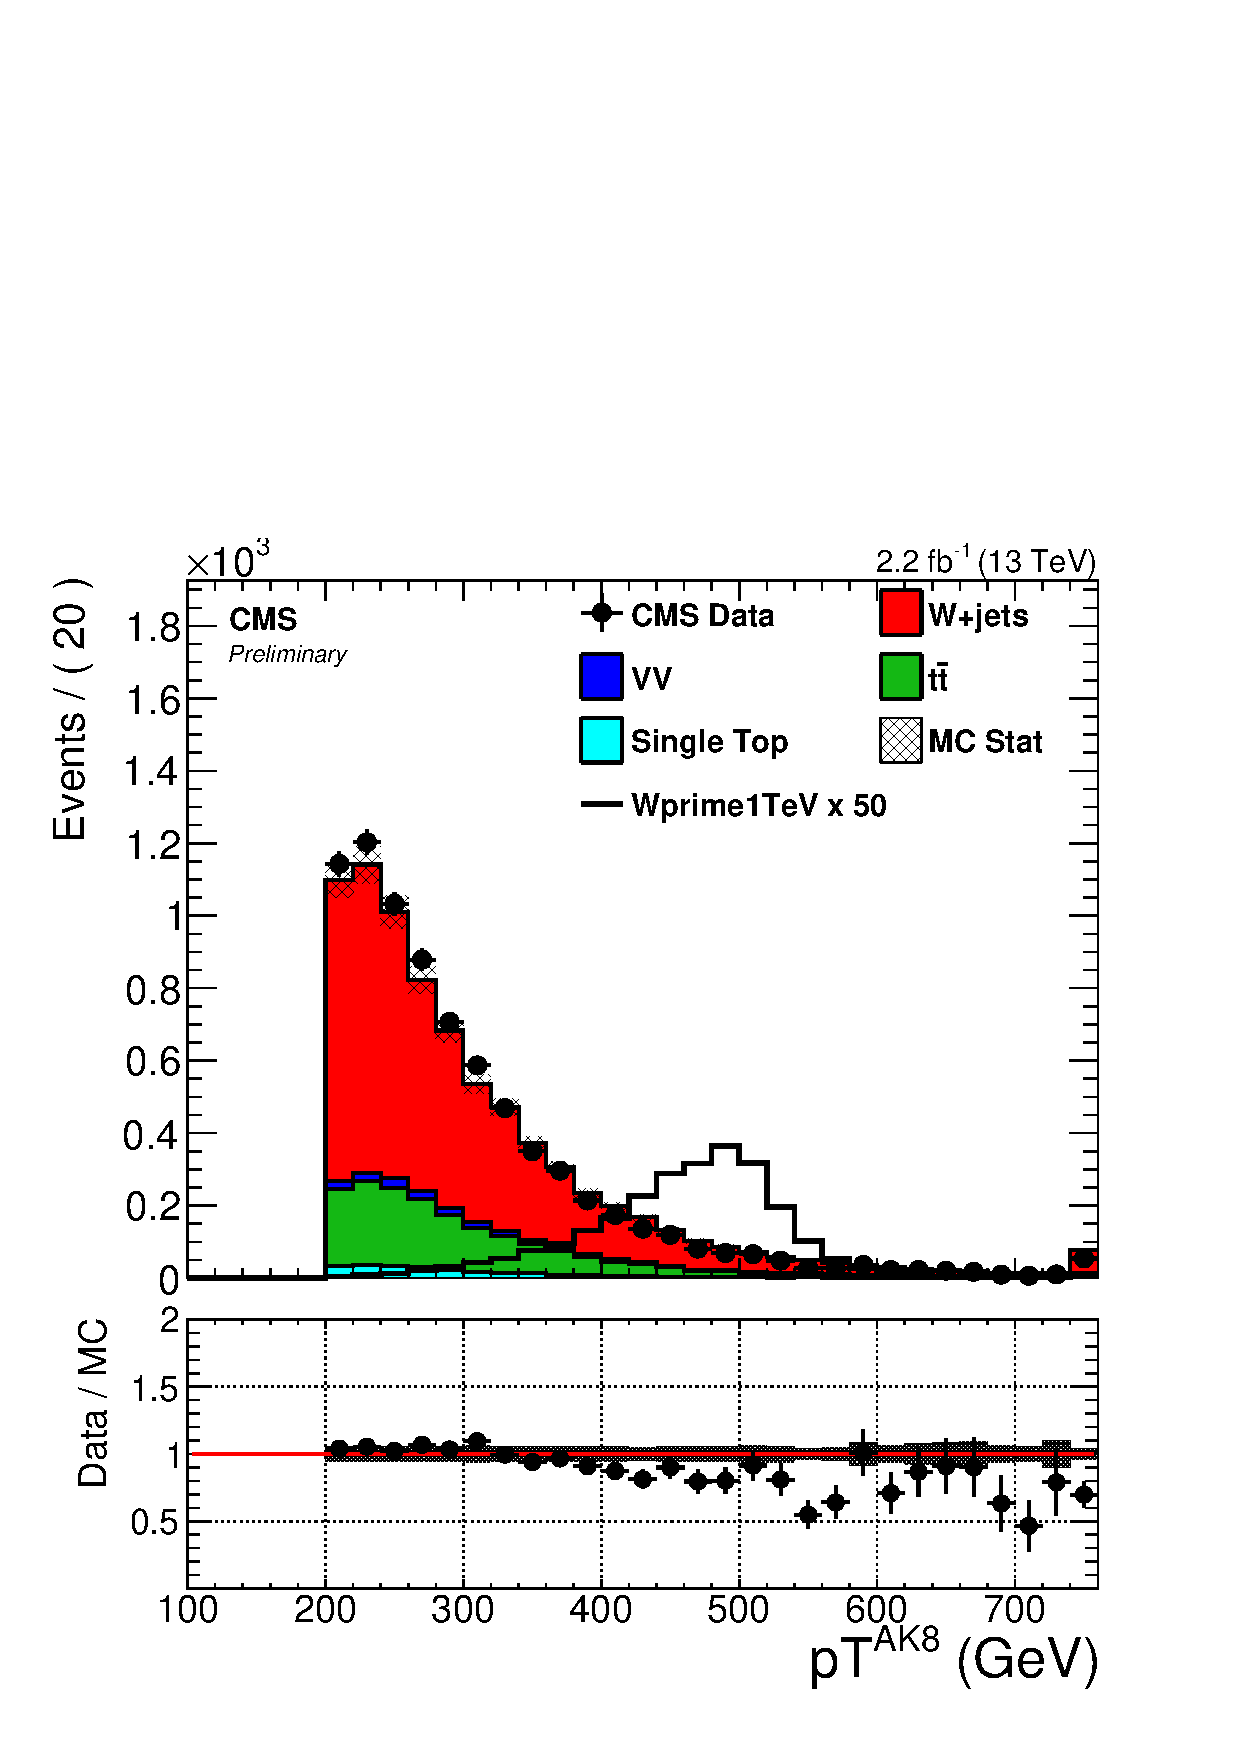
\includegraphics[width=0.45\textwidth]{\cheight/ptvjet-13TeV-wjets.pdf}}
\subfigure[]{\label{fig:controlPlots13TeV_b}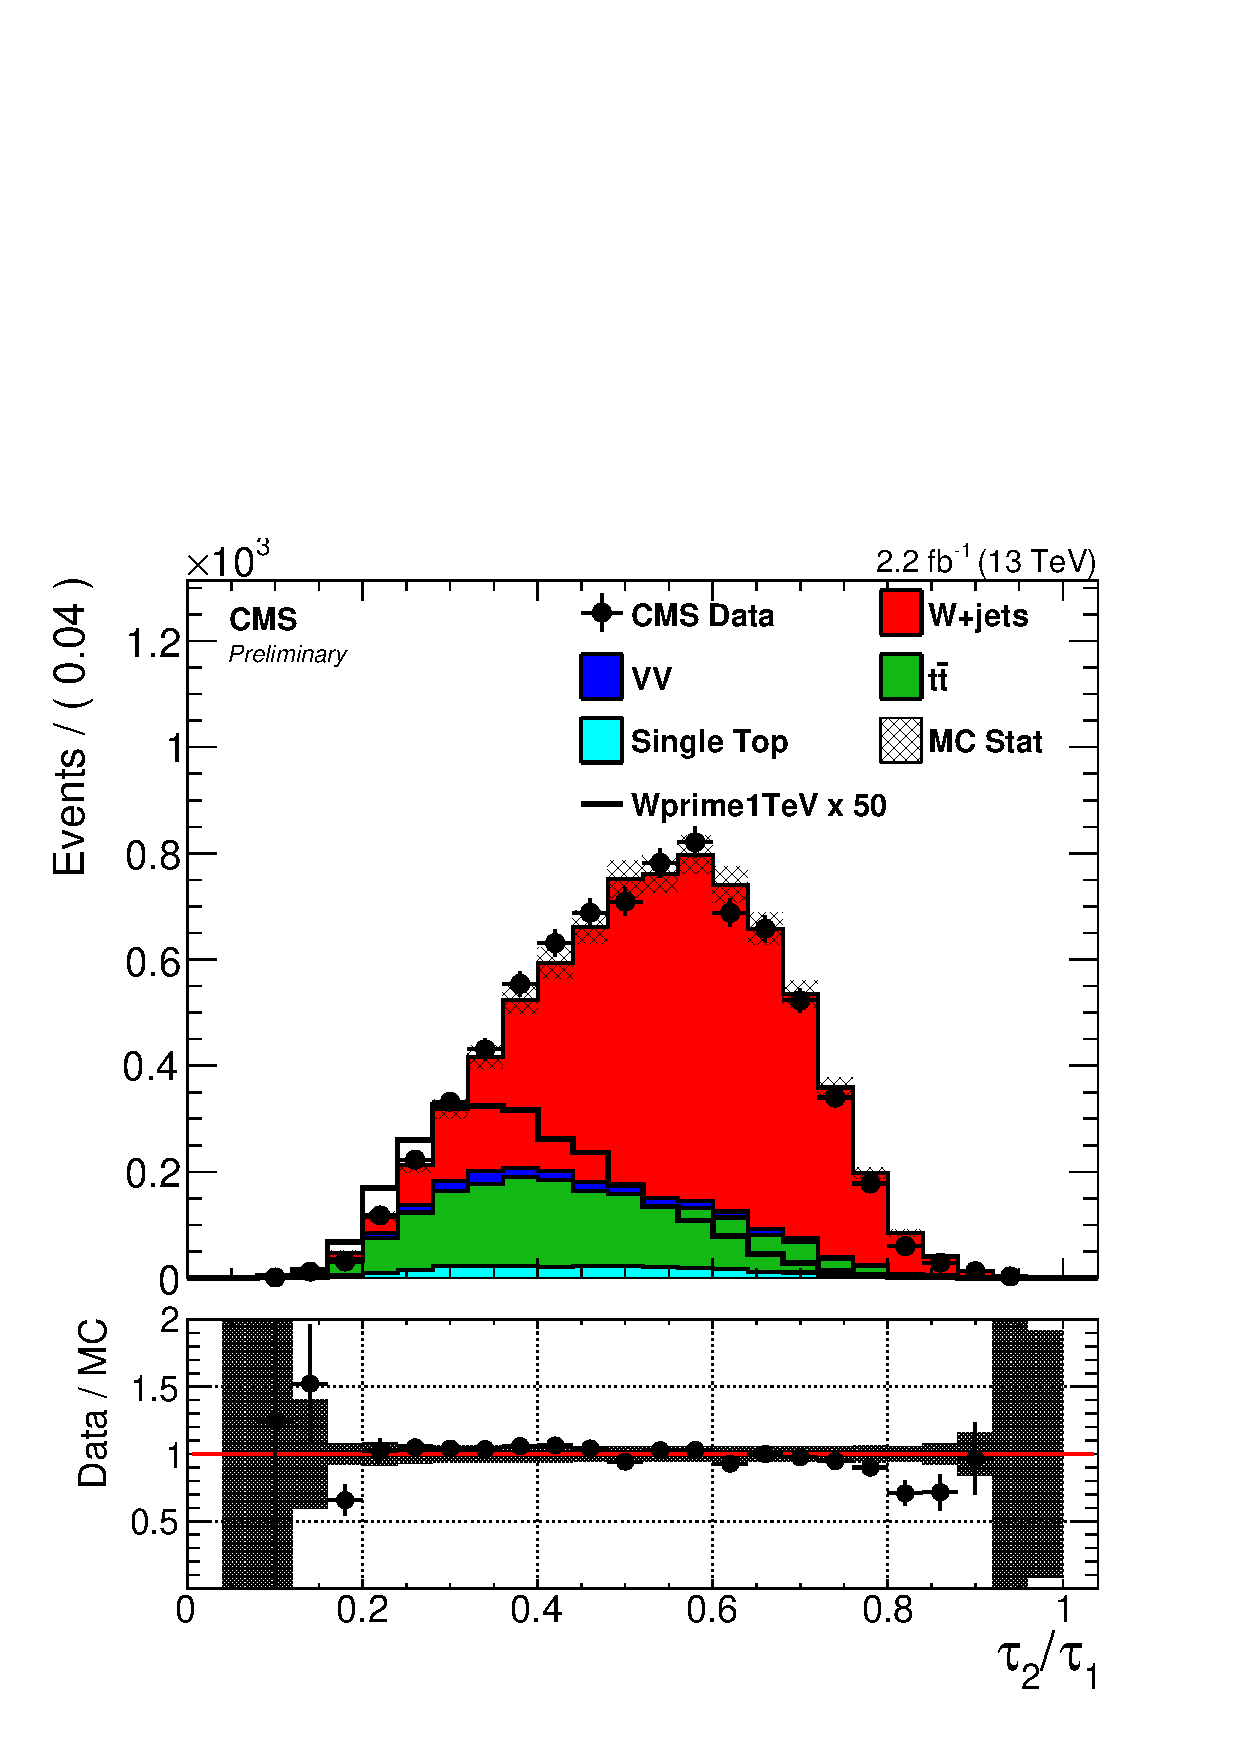
\includegraphics[width=0.45\textwidth]{\cheight/tau21-13TeV-wjets.pdf}}
\caption{Distributions in \pt (a) and N-subjettiness ratio \nsubj (b) for the V-jet candidate obtained requiring $65 < \mJ < 105\GeV$ after merging muon and electron channels. The SM diboson, \ttbar, and single-top-quark backgrounds are taken from simulation and are normalized to the integrated luminosity of the 13\TeV data sample. The W+jets background is rescaled to match the number of events in data.}
\label{fig:controlPlots13TeV}
\end{figure}

\begin{figure}[!htb]
\centering
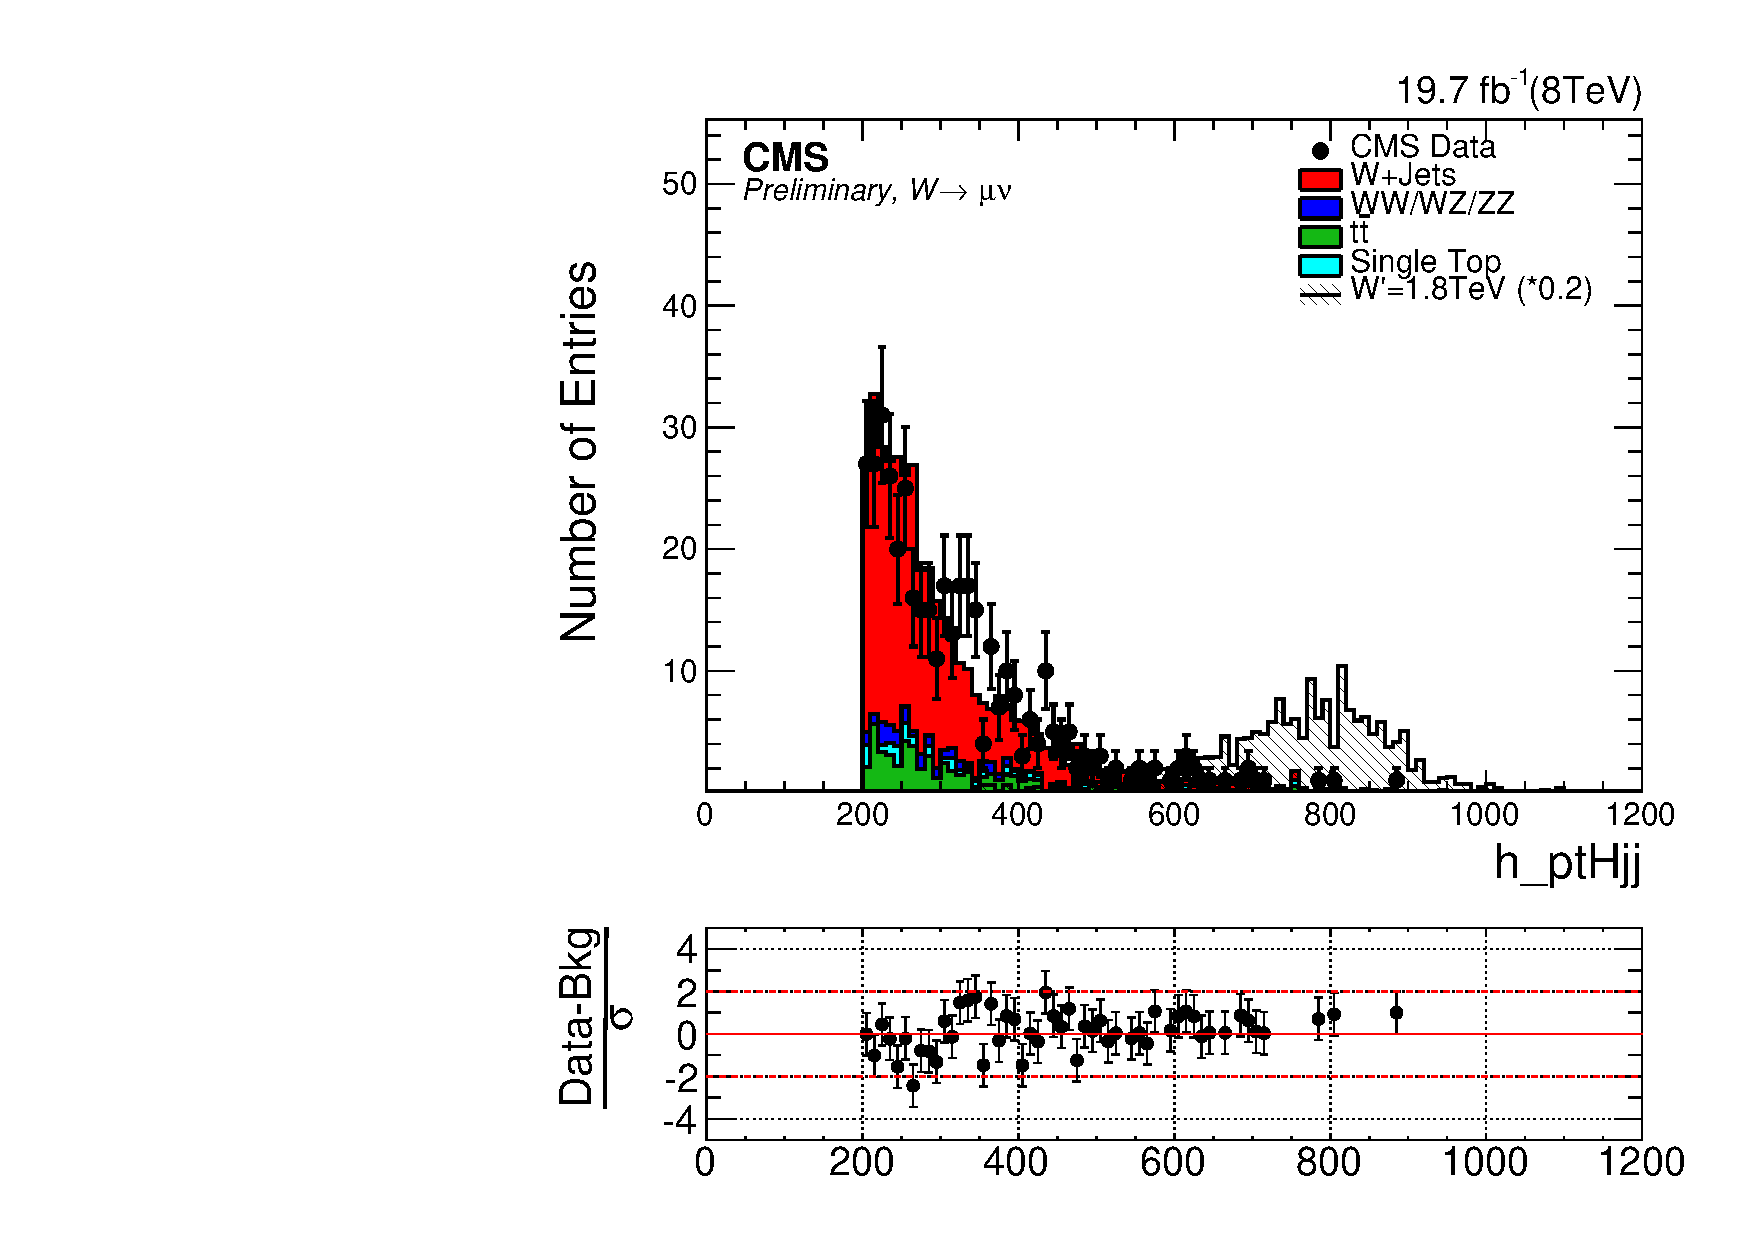
\includegraphics[width=0.5\textwidth]{\cheight/can_h_ptHjj.pdf}
\caption{Distributions in \pt for the H-jet candidate obtained requiring $40 < \mJ < 110\GeV$ for events in the muon channel. The SM diboson, \ttbar, and single-top-quark backgrounds are taken from simulation and are normalized to the integrated luminosity of the 8\TeV data sample. The W+jets background is rescaled to match the number of events in data.}
\label{fig:controlPlots8TeV}
\end{figure}